%--------------------------------------------------------------------------
% !TEX root = 5Blman.tex
% optical.tex
% 2013.01.06 changed to 2col format
%--------------------------------------------------------------------------
\chapter{Optical Instruments}

\begin{multicols}{2}
%---------------------------------------------------------------------
\section{Objective}
To apply the principles of angular magnification and lateral magnification to the astronomical refracting telescope and the compound microscope. Both the telescope and the microscope utilize the lens systems called the eyepiece (near the viewing eye) and the objective (near the object being magnified).

%---------------------------------------------------------------------
\section{The eyepiece} For this experiment the eyepiece will consist of a single converging lens which we will call a ``simple magnifier'' The simple magnifier magnifies an object by creating a virtual image which subtends a greater angle at the eye than the original object.

%\begin{figure} %{wrapfigure}[8]{r}[30pt]{3cm}	
%  \centering
%  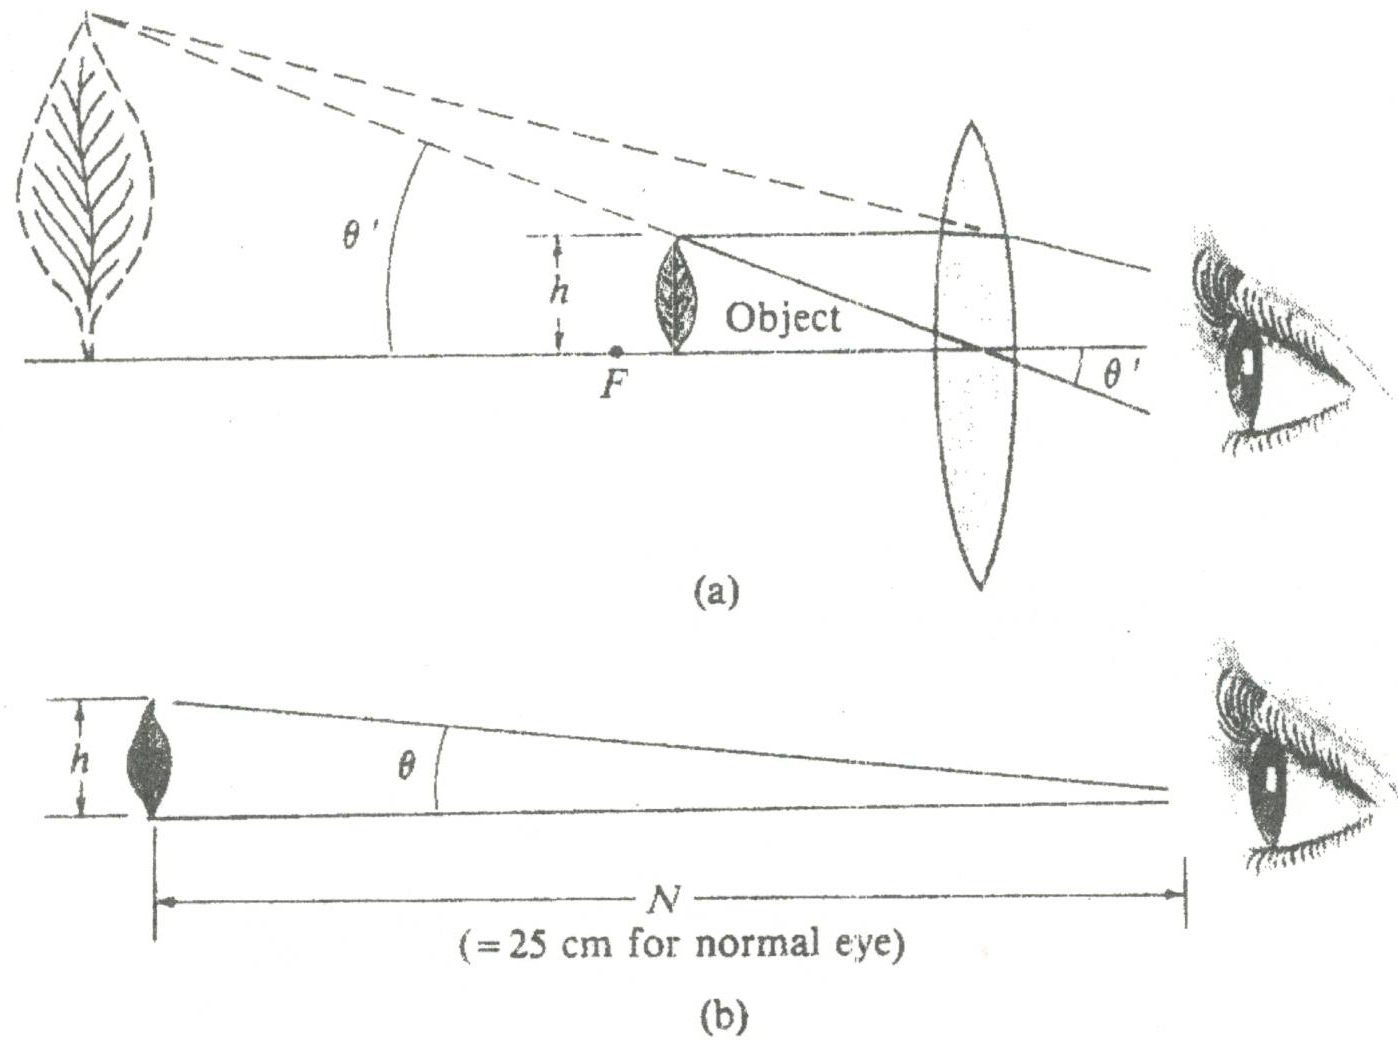
\includegraphics[scale=0.7]{5bgraf/mag}
%  \caption{Leaf viewed (a)through a magnifier (b)with the unaided eye}
%  \label{f:mag}
%\end{figure} %{wrapfigure}

\begin{center}
  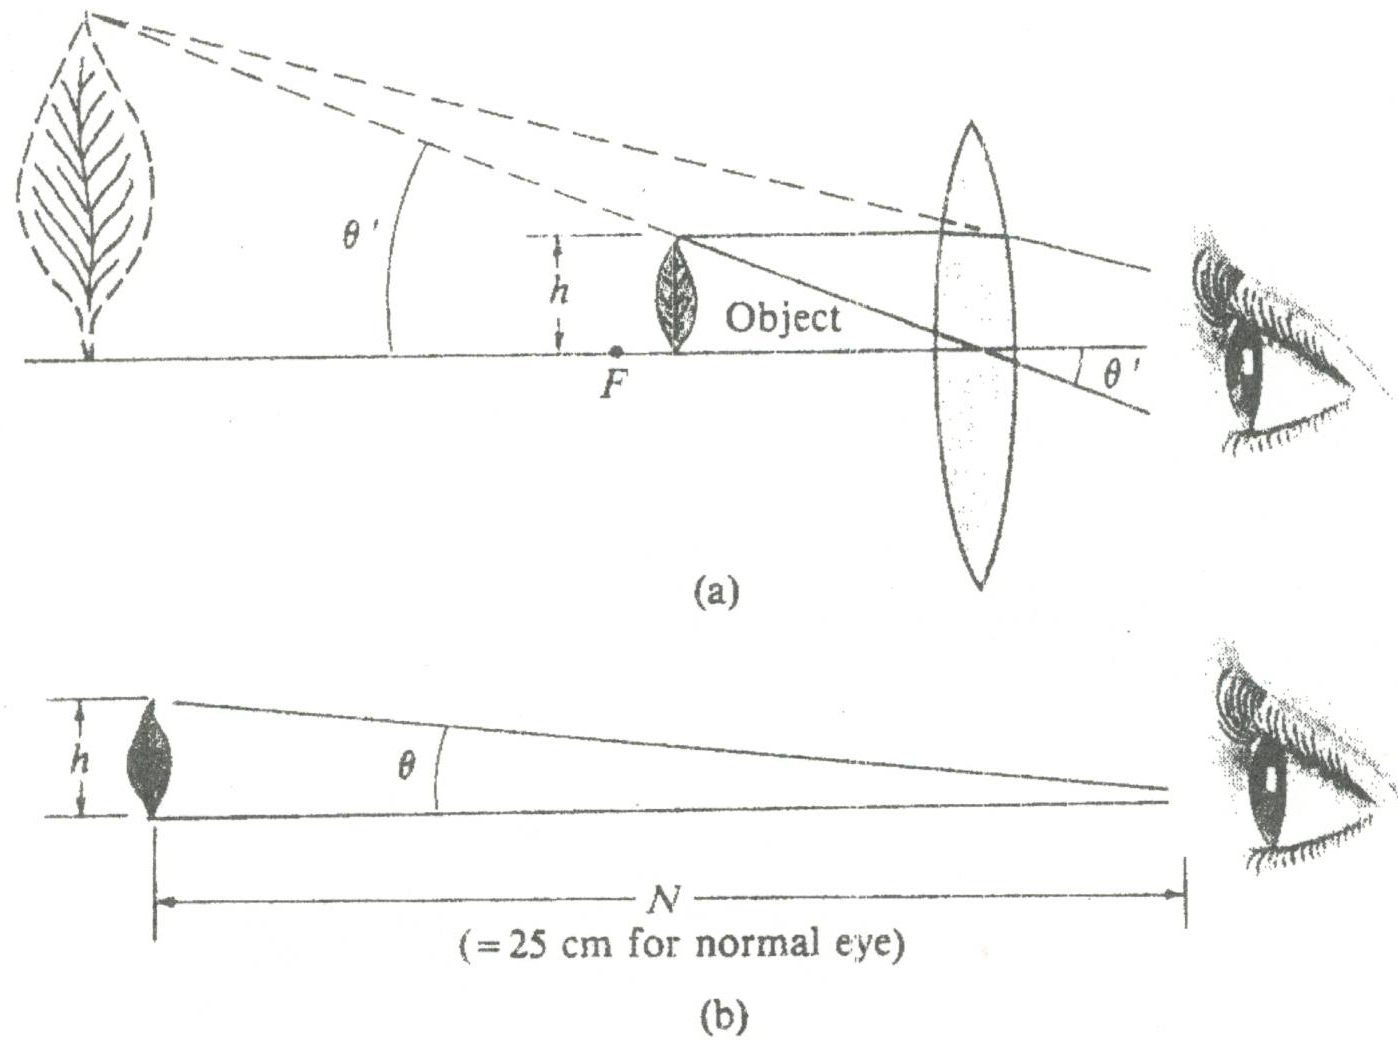
\includegraphics[scale=0.7]{5bgraf/mag}
  \mfcaption{Leaf viewed (a)through a magnifier (b)with the unaided eye}
  \label{f:mag}
\end{center}


This results in a larger image on the retina, hence the object ``appears'' larger. The amount the object appears to be larger is defined by the angular magnification or magnifying power of the lens.

For a normal eye (the near point, N = 25 cm)

% following are 3 methods to align math expression on more than 1 line
% alignment with the case environment
%\begin{equation}\label{e:mag}
%	M_{angular} = M_{eyepiece} =	
%	\begin{cases}
%		\frac{25}{f_e}		& \text {eye focused at infinity}\\
%		\frac{25}{f_e} + 1 	& \text {eye focused at near point (25 cm)}\\
%	\end{cases}
%\end{equation}

%% alignment with the array environment. specify #cols in array
%\begin{equation}
%	M_{angular} = M_{eyepiece} =
%	\left\{
%	\begin{array}{ll}
%		\frac{25}{f_e}		& \text {eye focused at infinity}\\
%		\frac{25}{f_e} + 1 	& \text {eye focused at near point (25 cm)}\\
%	\end{array}
%	\right.
%\end{equation}

% alignment with the alignedat environment. fractions are larger
\begin{equation}\label{e:mag}
	M_{angular} = M_{eyepiece} =
	\left\{
	\begin{alignedat}{2}
		&\frac{N}{f_e}		&& \quad\text {eye focused at infinity}\\
		&\frac{N}{f_e} + 1 	&& \quad\text {eye focused at near point}\\
	 \end{alignedat}
	\right.
\end{equation}


$f_e$ = focal length of the simple magnifier eyepiece

Note: Images formed by the eyepiece are virtual and upright, hence a simple magnifier can be used for reading purposes.

%---------------------------------------------------------------------
\section{The Refracting Astronomical Telescope}
A simple refracting telescope is illustrated in \reffig{f:tscope}

%\begin{figure}[htb] %{wrapfigure}[10]{r}[30pt]{3cm}	
%  \centering
%  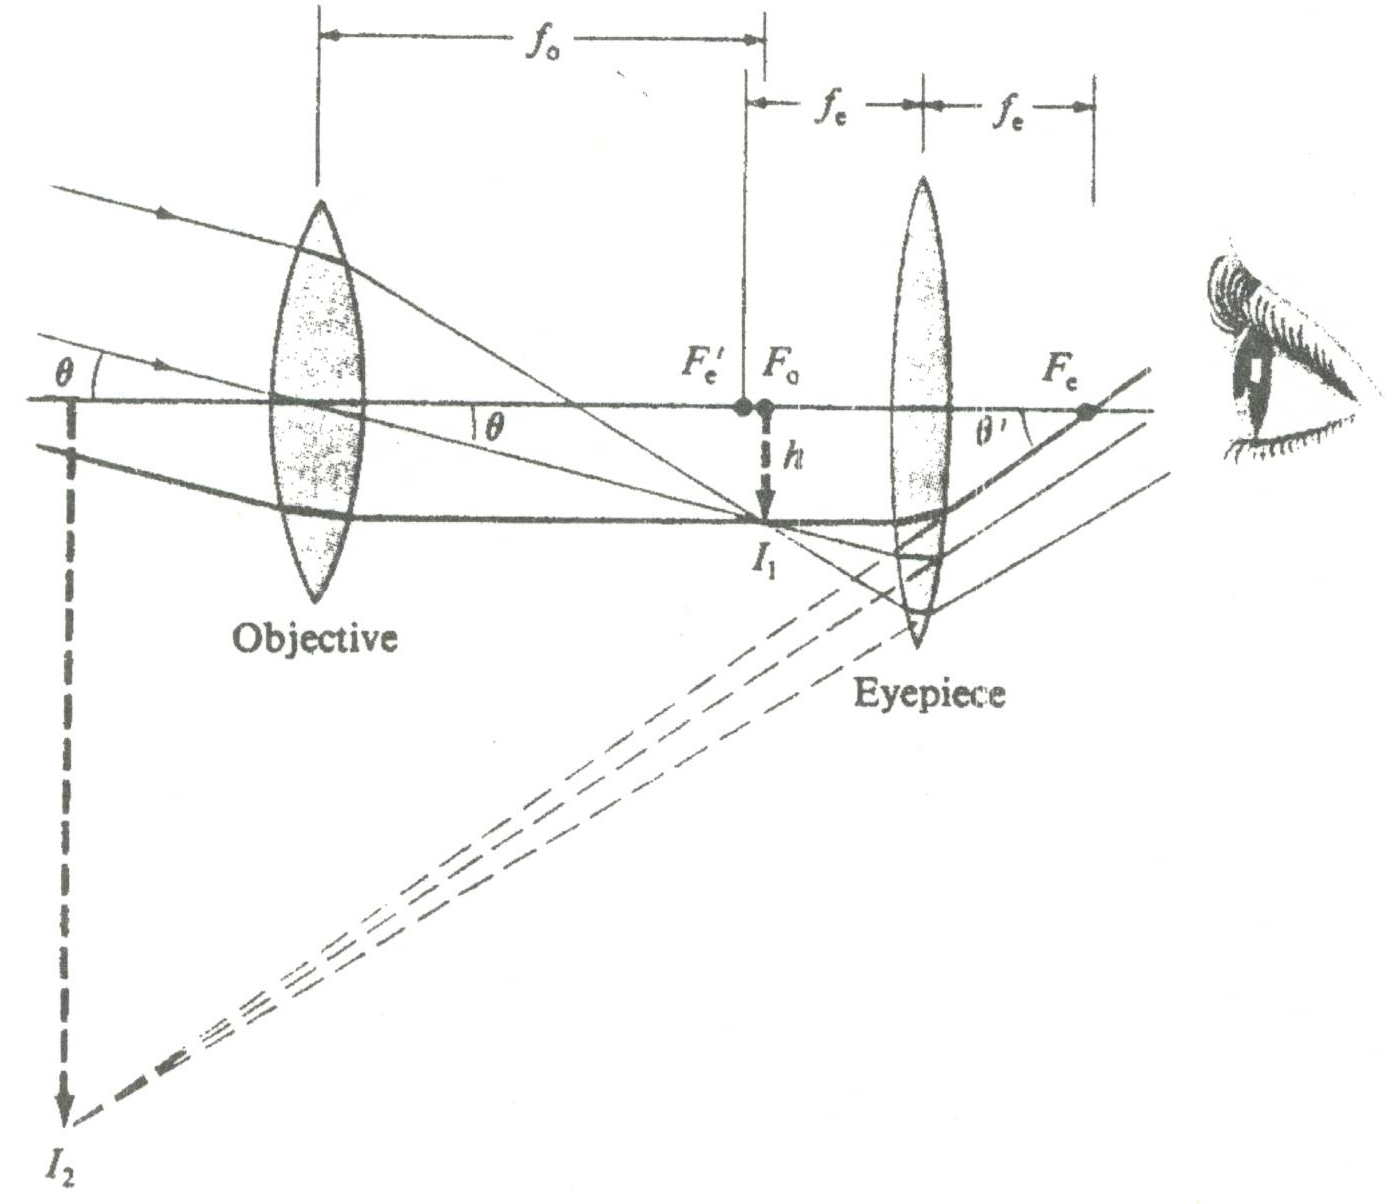
\includegraphics[scale=0.7]{5bgraf/tscope}
%  \caption{Refracting telescope}
%  \label{f:tscope}
%\end{figure} %{wrapfigure}

\begin{center}
  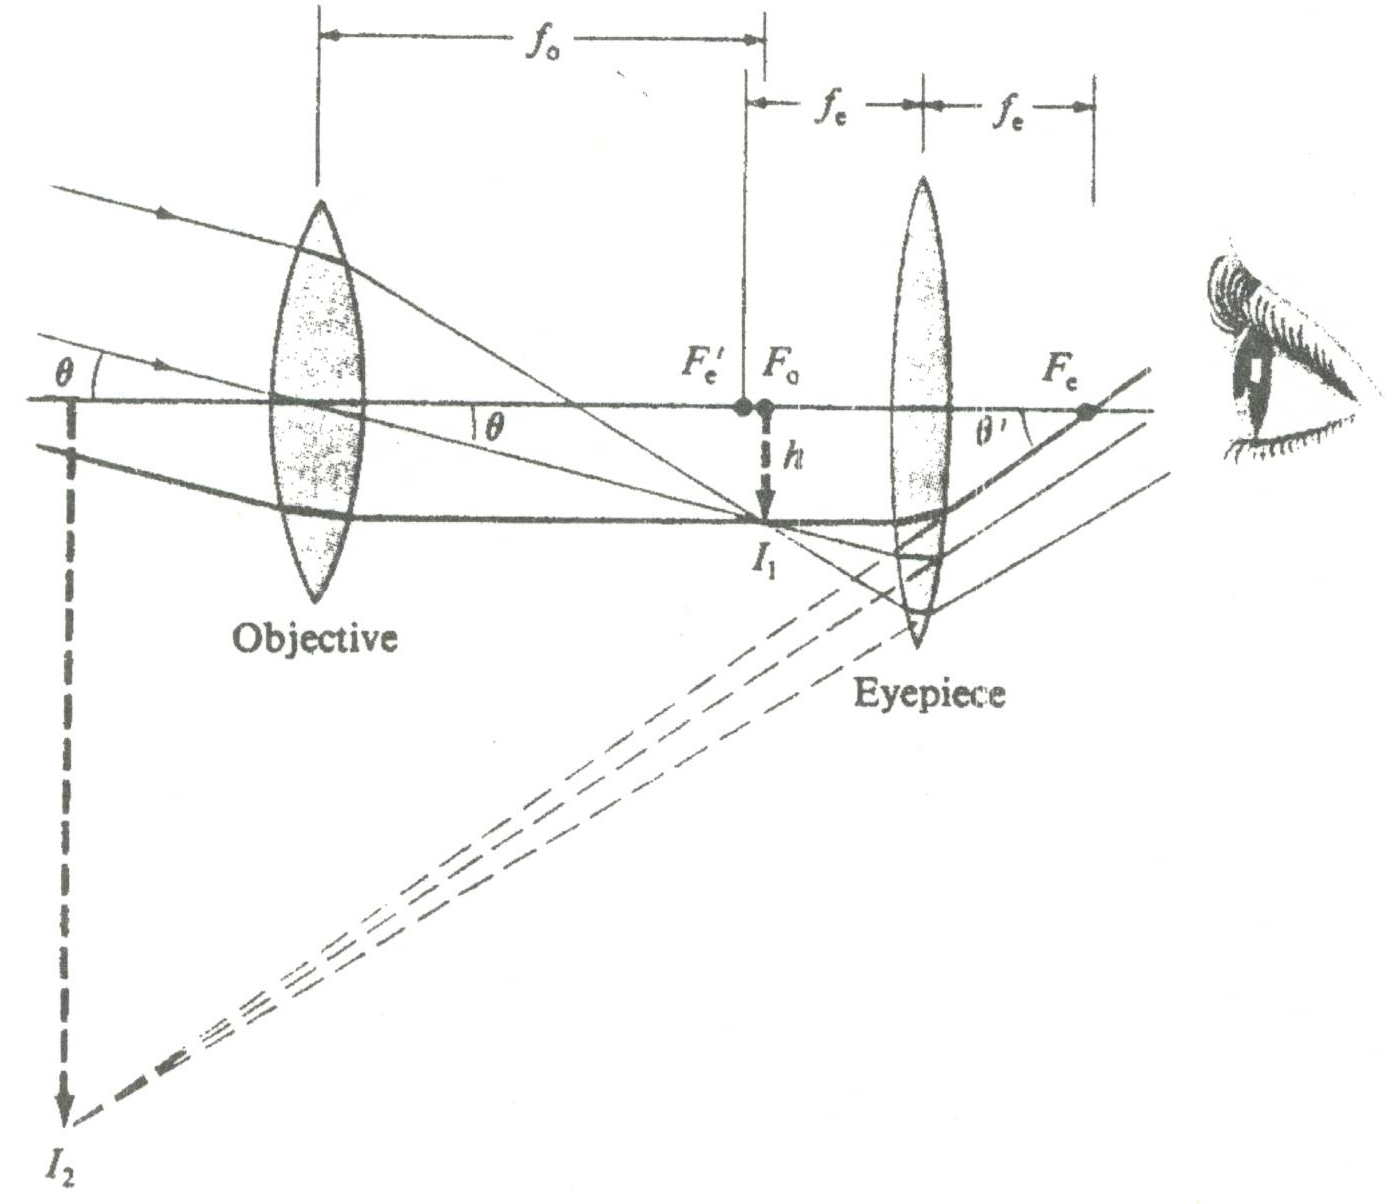
\includegraphics[scale=0.7]{5bgraf/tscope}
  \mfcaption{Refracting telescope}
  \label{f:tscope}
\end{center}


The features of this device are outlined as follows:
\begin{enumerate}
	\item The object is considered to be at infinity (very large distance). 
	\item The objective lens of focal length $f_o$ is of relatively large focal length.	
	\item The objective lens is a positive or converging lens.
	\item The objective lens forms a real, inverted image, which is then examined with the aid of the eyepiece lens, of focal length $f_e$. 
	\item The eyepiece lens is usually a short focal length lens.
	\item The eyepiece is then used to form a virtual image, at either the near point of the eye, or at infinity.
\end{enumerate}

Using trigonometric approximations you can confirm that the total magnifying power of this telescope is:
\begin{equation}\label{e:tscope}
	M = \frac{-f_o}{f_e}
\end{equation}
where the minus sign indicates that the image is `inverted'. It is assumed that the final image is at infinity.

\section{The Compound Microscope}
A simple compound microscope is illustrated in \reffig{f:mscope}:

%\begin{figure} [htb] %{wrapfigure}[8]{r}[20pt]{5cm}	
%  \centering
%  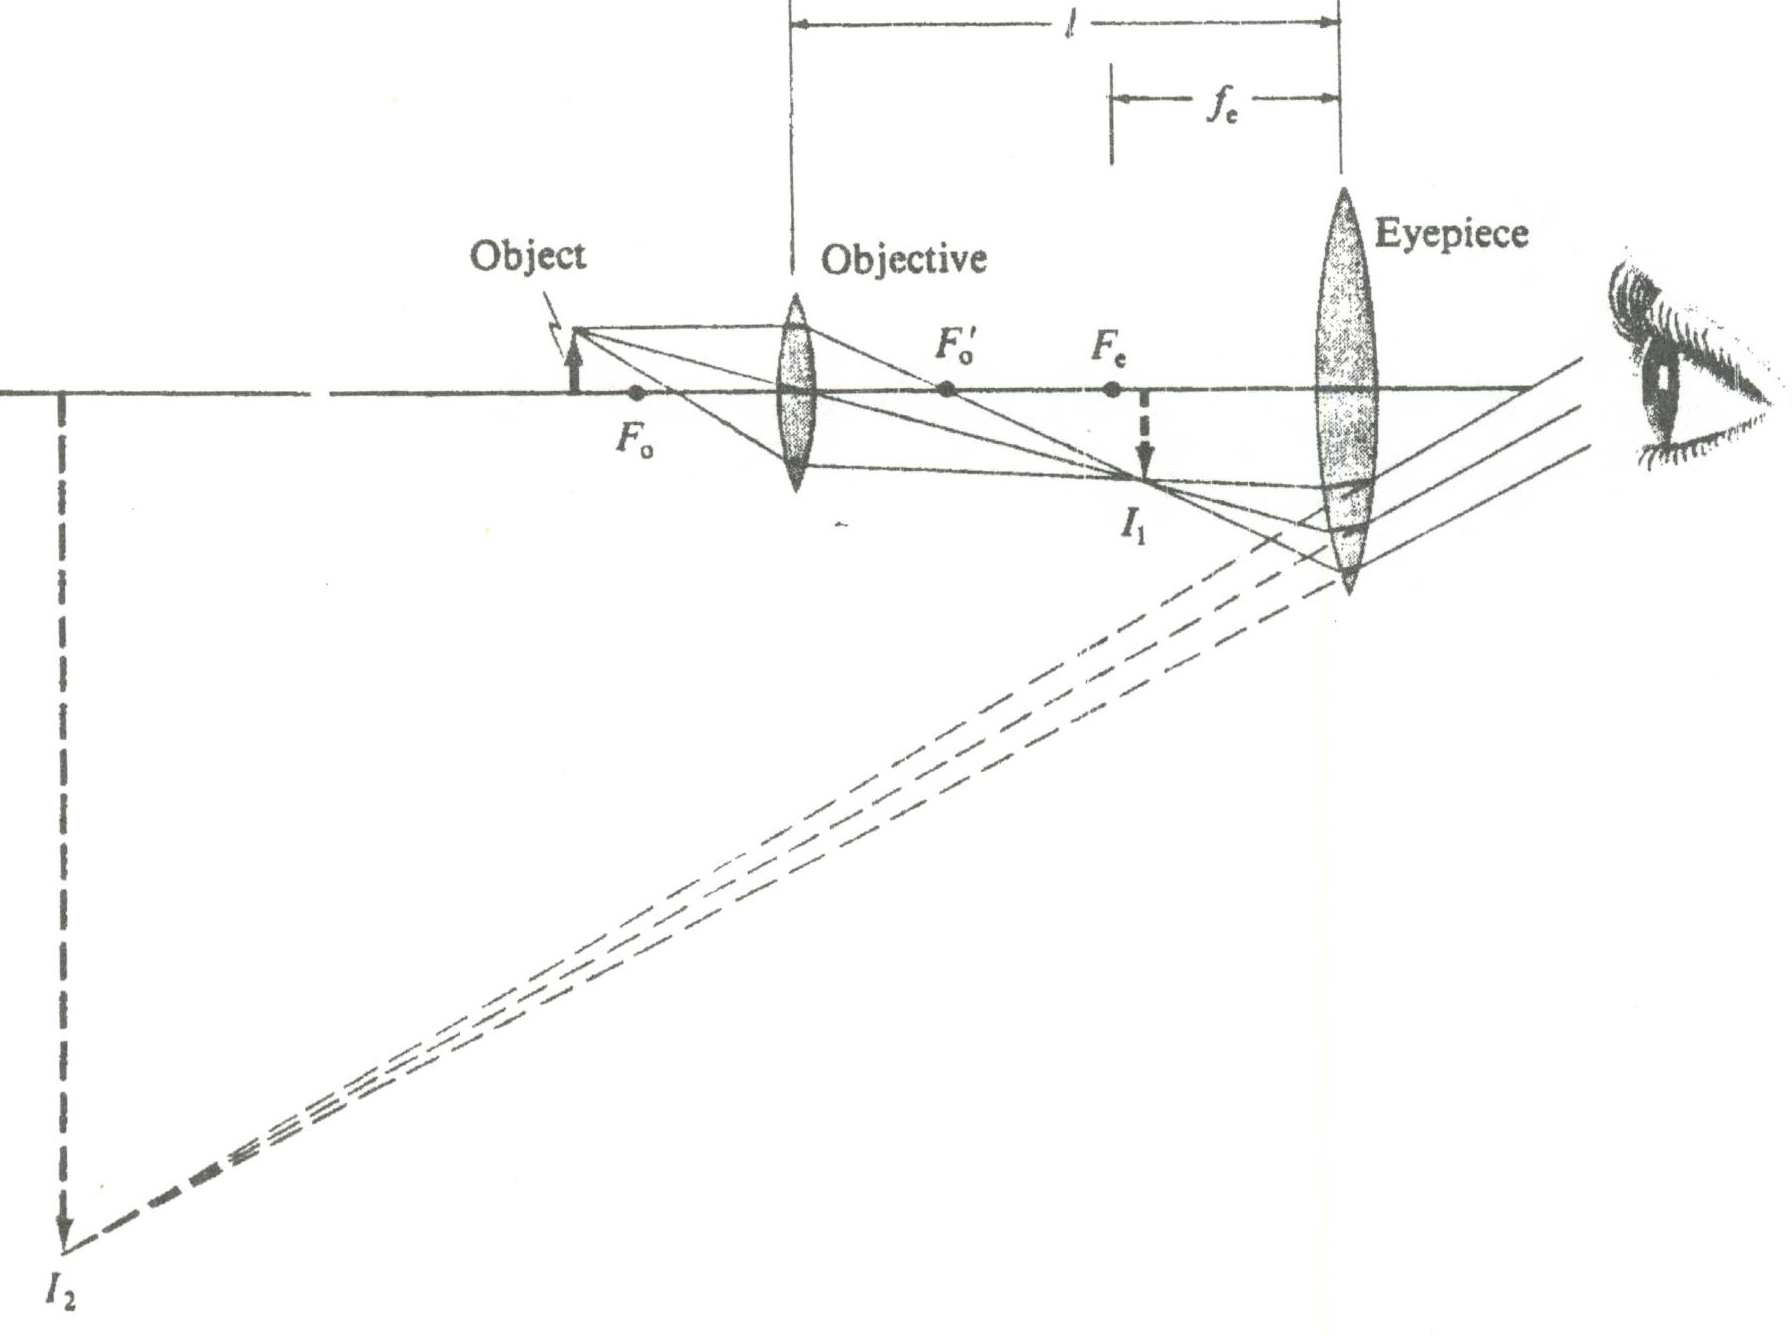
\includegraphics[scale=0.6]{5bgraf/mscope}
%  \caption{Compound microscope}
%  \label{f:mscope}
%\end{figure} %{wrapfigure}

\begin{center}
  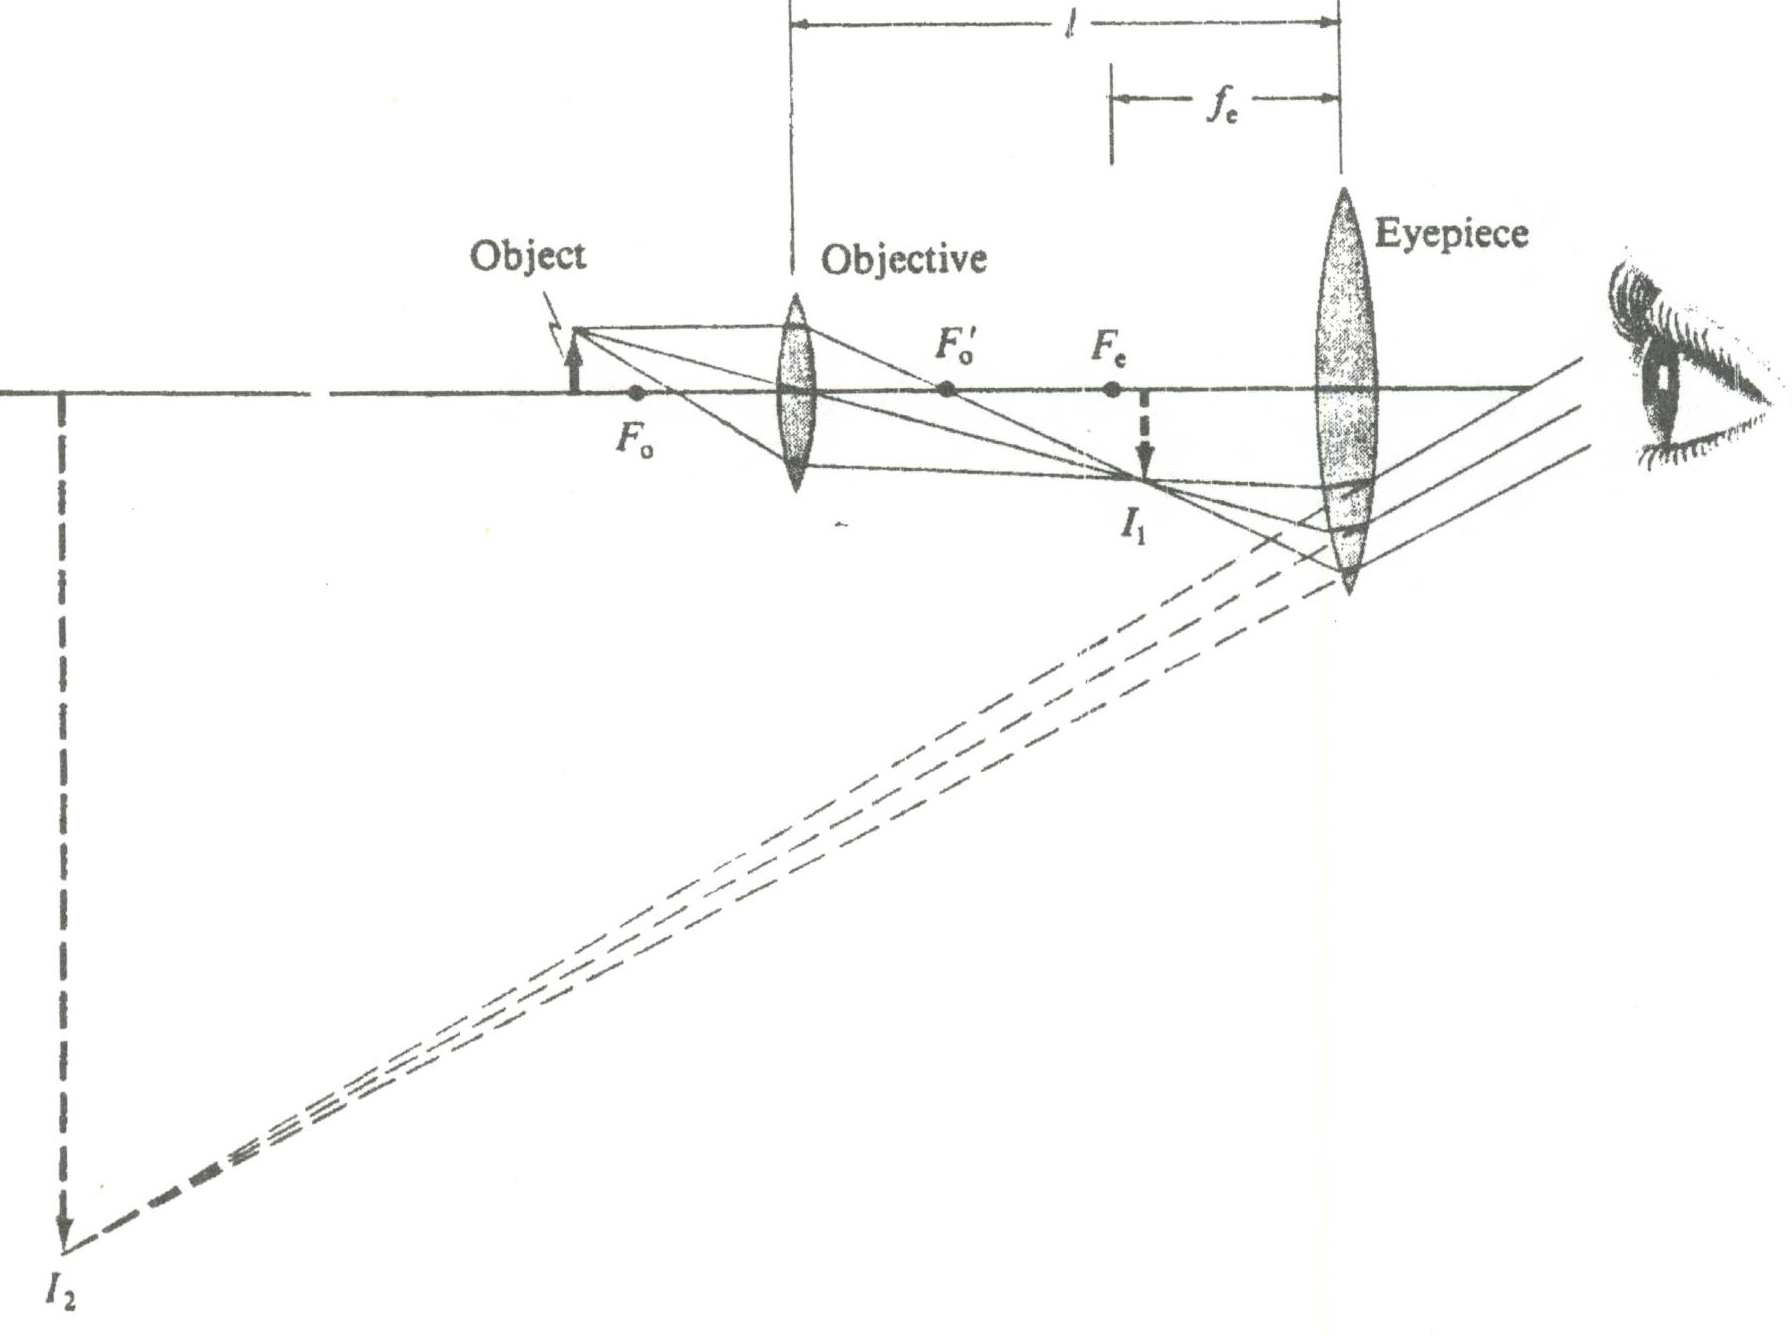
\includegraphics[scale=0.6]{5bgraf/mscope}
  \mfcaption{Compound microscope}
  \label{f:mscope}
\end{center}


The features of this device are outlined as follows:
\begin{enumerate}
	\item The object is located close to, but just outside the focal point of the objective lens.
	\item The objective lens is a short focal length lens.
	\item The objective lens is a positive or converging lens. 
	\item The lateral magnification of the objective lens is
	\[
		M_o = \frac{L-f_e }{d_o}\approx -\frac{L}{f_o}
	\] 
	where $d_o$ is the object distance.
\end{enumerate}

Thus, the overall magnification of the microscope is
\begin{equation} \label{e:mscope}
	M = M_o \cdot M_e = -\frac{L}{f_o}\frac{N}{f_e}
\end{equation}


%---------------------------------------------------------------------
\section{Building optical instruments}
\subsection{Activity: Find the focal lengths}
\begin{enumerate}
	\item You have been provided with three lenses of different focal lengths.  Hold each lens up to a bright distant source of light (room lights out, focusing upon a distant object outdoors), and form a real image on a sheet of plain paper. Find, as accurately as possible, the distance from the image to the lens. This distance is a fairly accurate measure of the focal length of the lens. Recall that the focal length of a positive thin lens is that point where light from infinity is brought to focus. 

	\item Identify which lens you will use as an eyepiece or simple magnifier, and which lens will serve as an objective lens for the telescope and which for the microscope objective. Both the telescope and the microscope will utilize the same eyepiece lens.
\end{enumerate}

\subsection{Activity: Simple magnifier}
\begin{enumerate}
	 \item Mount a ruler in a vertical position on the optical bench. Use the simple magnifier to observe the magnified image of the ruler markings, as seen through the simple magnifier.
	 \item  Devise a way to measure the size of the image seen through the magnifier. Then compare the actual size of the ruler marking with the size as seen through the simple magnifier. 
	 \item Compare your experimental observations with that predicted from equations in \refeqn{e:mag}.
\end{enumerate}

\subsection{Activity: Build a telescope}
% On the optical bench, set up an astronomical telescope. Sight on a distant object (out the window or in the lab) of known or approximate size, and estimate the magnification observed. Compare with results predicted by equation \ref{e:tscope}.
 
\begin{enumerate}
	\item Mount your eyepiece and objective lens for your telescope on your optical bench. Remember that you need an objective lens with a long focal length for a telescope. The distance between your lenses should be about the sum of their focal lengths.
	\item Sight your telescope on a distant object (on the other side of the room or outside). You might need to adjust the separation of your lenses to get a good image. 
	\item Estimate the magnification of the image, and then compare your results with the expected angular magnification, predicted by \refeqn{e:tscope}.
\end{enumerate}

\subsection{Activity: Build a microscope}
%On the optical bench, set up a simple microscope. From the known size of the object, and the estimated size of the image seen, find the overall magnification produced. Compare your observed value with that calculated from equation \ref{e:mscope}. Make use of both values of possible magnification for the eyepiece.

\begin{enumerate}
	\item Mount your eyepiece and objective lens for your microscope on your optical bench. Remember that you need an objective lens with a short focal length for a microscope. The distance between your lenses should be longer than the sum of their focal lengths.
	\item Sight your microscope on a small object placed near the objective, just outside of the focal length of the objective. The distance scale on your screen is one possible object to start with. Again, estimate the overall magnification for your microscope and compare it with the expected value predicted by \refeqn{e:mscope}.
\end{enumerate}

%---------------------------------------------------------------------
\section{Question} 
The size of the image of Jupiter as seen through a telescope is definitely
smaller than the actual planet, ($h_{image} < h_{object}$ ), yet we say that the telescope has provided magnification. Explain what is being magnified.

\end{multicols}
%--------------------------------------------------------------------------
\endinput
%--------------------------------------------------------------------------
